\documentclass[tikz,border=10pt]{standalone}
\usepackage{amsmath}
\usepackage{amssymb}
\usepackage{tikz}
\usetikzlibrary{arrows.meta,calc}

\definecolor{figazul}{RGB}{2,132,199}
\definecolor{figrojo}{RGB}{220,38,38}
\definecolor{figverde}{RGB}{22,163,74}

\begin{document}
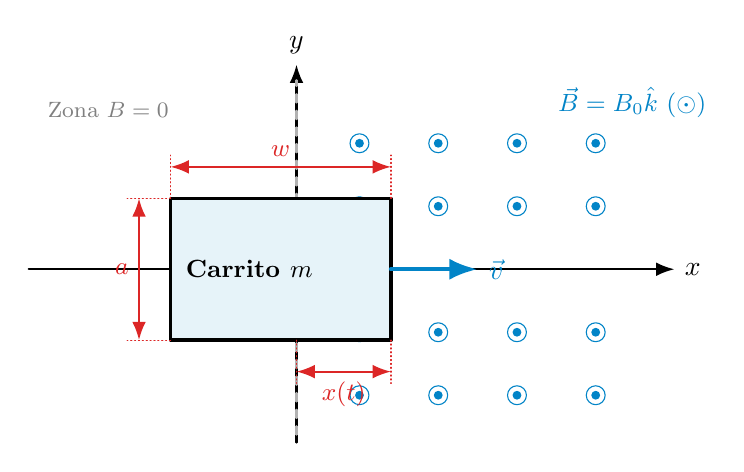
\begin{tikzpicture}[>=Latex, line cap=round, line join=round]
  % Ejes coordenados x, y
  \draw[->, thick] (-3.4, 0) -- (4.8, 0) node[right] {$x$};
  \draw[->, thick] (0, -2.2) -- (0, 2.6) node[above] {$y$};
  \node[below left] at (0,0) {$O$};

  % Frontera x = 0 (línea discontinua que separa zona B=0 de zona B)
  \draw[dashed, thick, color=gray!60] (0, -2.1) -- (0, 2.4);

  % Campo magnético uniforme B = B_0 k_hat (\odot) en x >= 0
  \foreach \gx in {0.8, 1.8, 2.8, 3.8} {
    \foreach \gy in {-1.6, -0.8, 0.8, 1.6} {
      \draw[thin, color=figazul] (\gx, \gy) circle (0.12);
      \fill[color=figazul] (\gx, \gy) circle (1.6pt);
    }
  }
  \node[above right, font=\small, color=figazul] at (3.2, 1.8) {$\vec{B} = B_0\hat{k}$ ($\odot$)};
  \node[above left, font=\footnotesize, color=gray] at (-1.5, 1.8) {Zona $B = 0$};

  % Carrito conductor rectangular de dimensiones w x a ingresando a la zona con campo
  % Supongamos w = 2.8, a = 1.8.
  % Parte dentro: de x = 0 a x = 1.2 (longitud penetrada x(t) = 1.2)
  % Parte fuera: de x = -1.6 a x = 0
  % y va de -0.9 a +0.9 (ancho a = 1.8)
  \draw[very thick, fill=figazul!10] (-1.6, -0.9) rectangle (1.2, 0.9);

  % Ruedas simbólicas o masa m
  \node[font=\small\bfseries] at (-0.6, 0) {Carrito $m$};

  % Vector velocidad v hacia +x
  \draw[->, ultra thick, color=figazul] (1.2, 0) -- (2.3, 0) node[right, color=figazul] {$\vec{v}$};

  % Cotas en rojo
  % Cota a (ancho vertical)
  \draw[<->, thick, color=figrojo] (-2.0, -0.9) -- (-2.0, 0.9) node[midway, left, color=figrojo, font=\small] {$a$};
  \draw[densely dotted, thin, color=figrojo] (-1.6, -0.9) -- (-2.15, -0.9);
  \draw[densely dotted, thin, color=figrojo] (-1.6, 0.9) -- (-2.15, 0.9);

  % Cota w (largo total del carrito)
  \draw[<->, thick, color=figrojo] (-1.6, 1.3) -- (1.2, 1.3) node[midway, above, color=figrojo, font=\small] {$w$};
  \draw[densely dotted, thin, color=figrojo] (-1.6, 0.9) -- (-1.6, 1.45);
  \draw[densely dotted, thin, color=figrojo] (1.2, 0.9) -- (1.2, 1.45);

  % Cota x(t) de la porción dentro del campo magnético
  \draw[<->, thick, color=figrojo] (0, -1.3) -- (1.2, -1.3) node[midway, below, color=figrojo, font=\small] {$x(t)$};
  \draw[densely dotted, thin, color=figrojo] (0, -0.9) -- (0, -1.45);
  \draw[densely dotted, thin, color=figrojo] (1.2, -0.9) -- (1.2, -1.45);

\end{tikzpicture}
\end{document}
